\documentclass[]{standalone}
\usepackage{tikz}
\begin{document}
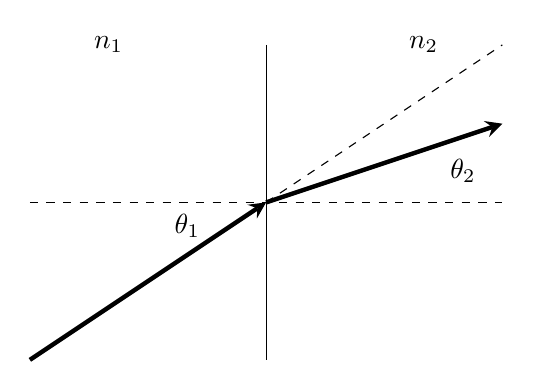
\begin{tikzpicture}
  \node(n1) at (0,0) {$n_1$};
  \node[right of = n1,node distance = 4cm](n2) {$n_2$};
  \draw (2,0) -- (2,-4);
  %Initial Ray
  \draw[->,>=stealth, line width = 1.6pt] (-1,-4) -- (2,-2); 
  % Ray without bending
  \draw[dashed] (2,-2) -- (5,0); 
  \draw[dashed] (-1,-2) -- (5,-2); 
  % Bent Ray
  \draw[->,>=stealth,line width = 1.6pt] (2,-2) -- (5,-1);
  \node(thetaone) at (1,-2.3) {$\theta_1$};
  \node(thetatwo) at (4.5,-1.6) {$\theta_2$};
\end{tikzpicture}
\end{document}
